\documentclass[12pt,a4paper]{article}
\usepackage[utf8]{inputenc}
\usepackage{amsmath, amssymb, amsfonts}
\usepackage{graphicx}
\usepackage{fullpage}
\usepackage{enumitem}
\usepackage{hyperref}
\usepackage{tikz}
\usetikzlibrary{shapes,arrows,positioning,fit,calc,matrix,decorations.pathreplacing}

\title{KUNCI JAWABAN UAS IF1220 MATEMATIKA DISKRIT}
\author{Kelas 3E Kunugigaoka Junior High School}
\date{}

\begin{document}

\noindent \textbf{Nama: Kalyca Nathania Benedicta Manullang} \\
\noindent \textbf{NIM: 13524071}
\vspace{0.3cm}

\maketitle

\begin{center}
\Large \textbf{BAGIAN A: SOAL MUDAH (EASY)}
\end{center}

\section*{Soal 1 Logika dan Penalaran}
\subsection*{Analisis}
Kita diminta membuktikan apakah Dodi ($D$) pasti bersalah berdasarkan empat premis yang diberikan. Untuk itu, kita harus melakukan penarikan kesimpulan menggunakan aturan-aturan logika yang sahih (valid).

\subsection*{Langkah 1: Definisikan Proposisi}
Kita beri simbol untuk setiap pernyataan sederhana:
\begin{itemize}
    \item $A$: Andi bersalah.
    \item $B$: Budi bersalah.
    \item $C$: Cici bersalah.
    \item $D$: Dodi bersalah.
\end{itemize}

\subsection*{Langkah 2: Tulis Premis dalam Bentuk Simbolik}
Dari soal, kita peroleh empat premis:
\begin{enumerate}
    \item $A \rightarrow B$ \quad (Jika Andi bersalah, maka Budi bersalah)
    \item $C \rightarrow D$ \quad (Jika Cici bersalah, maka Dodi bersalah)
    \item $A \lor C$ \quad (Andi bersalah atau Cici bersalah)
    \item $\neg B$ \quad (Budi tidak bersalah)
\end{enumerate}
Kesimpulan yang ingin kita uji kebenarannya adalah $D$ (Dodi bersalah).

\subsection*{Langkah 3: Proses Penarikan Kesimpulan}
Kita gunakan aturan-aturan logika sebagai berikut:

\begin{enumerate}
    \item Dari premis (4) kita tahu $\neg B$ adalah benar.
    \item Premis (1) menyatakan $A \rightarrow B$. Jika $B$ salah ($\neg B$), maka berdasarkan \textbf{Modus Tollens}, kita dapat menyimpulkan $\neg A$ (Andi tidak bersalah). Modus Tollens berbunyi: jika $P \rightarrow Q$ dan $\neg Q$, maka $\neg P$.
    \item Sekarang kita punya $\neg A$ (Andi tidak bersalah) dan premis (3), yaitu $A \lor C$ (Andi atau Cici bersalah). Karena Andi tidak bersalah, agar $A \lor C$ bernilai benar, maka $C$ harus benar. Ini adalah aturan \textbf{Disjungsi Silogisme}: dari $P \lor Q$ dan $\neg P$, maka $Q$.
    \item Kita sekarang punya $C$ (Cici bersalah). Premis (2) adalah $C \rightarrow D$. Dengan \textbf{Modus Ponens} (jika $P \rightarrow Q$ dan $P$, maka $Q$), kita simpulkan $D$ (Dodi bersalah).
\end{enumerate}

\subsection*{Kesimpulan}
Karena dari premis-premis yang diberikan kita berhasil menurunkan $D$ secara sahih menggunakan aturan logika, maka \textbf{Dodi pasti bersalah}. Tidak ada interpretasi lain yang memungkinkan.

\newpage
\section*{Soal 2 Himpunan}
\subsection*{Analisis}
Kita memiliki tiga himpunan: Python ($P$), Java ($J$), dan C++ ($C$). Total karyawan adalah 120. Kita diberikan irisan antar himpunan. Untuk mencari yang tidak menguasai ketiganya, kita bisa menghitung semua yang \emph{menguasai} setidaknya satu bahasa, lalu kurangkan dari total.

\subsection*{Langkah 1: Tentukan Nilai Irisan yang "Hanya"}
Diketahui $|P \cap J \cap C| = 10$. Maka:
\begin{itemize}
    \item $|P \cap J|$ saja $= 25 - 10 = 15$.
    \item $|P \cap C|$ saja $= 20 - 10 = 10$.
    \item $|J \cap C|$ saja $= 15 - 10 = 5$.
    \item $|P|$ saja $= 65 - (15 + 10 + 10) = 30$.
    \item $|J|$ saja $= 50 - (15 + 5 + 10) = 20$.
    \item $|C|$ saja $= 45 - (10 + 5 + 10) = 20$.
\end{itemize}

\subsection*{Langkah 2: Gambar Diagram Venn}
Berikut adalah diagram Venn yang menggambarkan data tersebut. Angka di dalam irisan menunjukkan jumlah karyawan \emph{hanya} pada daerah tersebut.

\begin{center}
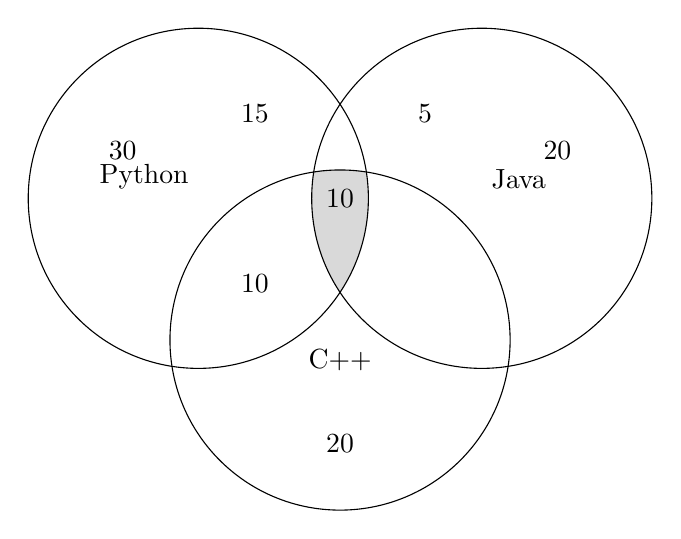
\begin{tikzpicture}[scale=1.2]
    \begin{scope}
        \clip (-1.5,0) circle (1.8);
        \clip (1.5,0) circle (1.8);
        \clip (0,-1.5) circle (1.8);
        \fill[gray!30] (-1.5,0) circle (1.8);
    \end{scope}
    
    % Draw circles
    \draw (-1.5,0) circle (1.8) node[above left] {Python};
    \draw (1.5,0) circle (1.8) node[above right] {Java};
    \draw (0,-1.5) circle (1.8) node[below] {C++};
    
    % Labels for regions
    \node at (-2.3,0.5) {30};   % P saja
    \node at (2.3,0.5) {20};    % J saja
    \node at (0,-2.6) {20};     % C saja
    \node at (-0.9,0.9) {15};   % P∩J saja
    \node at (0.9,0.9) {5};     % J∩C saja
    \node at (-0.9,-0.9) {10};  % P∩C saja
    \node at (0,0) {10};        % P∩J∩C
\end{tikzpicture}
\end{center}

\subsection*{Langkah 3: Hitung yang Tidak Menguasai Ketiganya}
Jumlah karyawan yang menguasai \emph{setidaknya satu} bahasa adalah jumlah semua bagian dalam diagram Venn:
$30 + 20 + 20 + 15 + 10 + 5 + 10 = 110$.

Total karyawan adalah 120. Maka yang tidak menguasai ketiga bahasa (yaitu tidak menguasai Python, tidak Java, dan tidak C++) adalah:
$120 - 110 = 10$ orang.

\subsection*{Jawaban Akhir}
\textbf{10 orang} karyawan tidak menguasai satupun dari ketiga bahasa tersebut.

\newpage
\section*{Soal 3 Relasi dan Fungsi}
\subsection*{Analisis}
Kita periksa tiga sifat relasi: Refleksif, Setangkup (Simetris), dan Menghantar (Transitif). Relasi $R$ didefinisikan pada himpunan $A = \{2,3,4,5\}$.

\subsection*{a) Refleksif}
\textbf{Definisi:} Relasi $R$ refleksif jika untuk setiap $a \in A$, pasangan $(a,a) \in R$.
Periksa elemen $A$:
\begin{itemize}
    \item $(2,2) \in R$ (ada)
    \item $(3,3) \in R$ (ada)
    \item $(4,4) \in R$ (ada)
    \item $(5,5) \in R$ (ada)
\end{itemize}
Karena semua elemen memiliki pasangan refleksif, maka $R$ \textbf{bersifat refleksif}.

\subsection*{b) Setangkup (Simetris)}
\textbf{Definisi:} Relasi $R$ setangkup jika untuk setiap $(a,b) \in R$ dengan $a \neq b$, maka $(b,a)$ juga harus ada di $R$.
Perhatikan pasangan $(2,4) \in R$. Jika $R$ setangkup, maka $(4,2)$ harus ada. Namun, $(4,2)$ \textbf{tidak ada} di dalam $R$. Ini sudah cukup untuk membuktikan bahwa $R$ \textbf{tidak setangkup}.

\subsection*{c) Menghantar (Transitif)}
\textbf{Definisi:} Relasi $R$ menghantar jika untuk setiap $(a,b) \in R$ dan $(b,c) \in R$, maka $(a,c) \in R$.
Kita periksa semua kemungkinan:
\begin{itemize}
    \item Ambil $(2,4)$ dan $(4,4)$ $\rightarrow$ $(2,4)$ ada $\checkmark$
    \item Ambil $(3,5)$ dan $(5,5)$ $\rightarrow$ $(3,5)$ ada $\checkmark$
    \item Tidak ada pasangan $(a,b)$ dan $(b,c)$ dengan $b$ berbeda yang menghasilkan pelanggaran.
\end{itemize}
Karena tidak ditemukan pelanggaran, maka $R$ \textbf{bersifat menghantar}.

\subsection*{Kesimpulan Akhir}
$a)$ Refleksif: Ya. \quad $b)$ Setangkup: Tidak. \quad $c)$ Menghantar: Ya. 

\newpage
\section*{Soal 4 Teori Bilangan}
\subsection*{Analisis}
Algoritma Euclidean adalah cara efisien untuk mencari FPB (GCD) dengan membagi bilangan yang lebih besar dengan yang lebih kecil secara berulang hingga sisa 0. FPB adalah sisa terakhir yang bukan nol. KPK (LCM) didapat dari rumus $\operatorname{lcm}(a,b) = \frac{a \cdot b}{\gcd(a,b)}$.

\subsection*{Langkah 1: Cari $\gcd(180, 72)$}
Terapkan algoritma pembagian:
\begin{align*}
180 &= 2 \times 72 + 36 \quad (\text{Sisa } 36) \\
72  &= 2 \times 36 + 0 \quad (\text{Sisa } 0, \text{berhenti})
\end{align*}
Sisa terakhir sebelum 0 adalah 36. Jadi, $\gcd(180,72) = 36$.

\subsection*{Langkah 2: Cari $\operatorname{lcm}(180, 72)$}
Gunakan rumus:
\[
\operatorname{lcm}(180,72) = \frac{180 \times 72}{\gcd(180,72)} = \frac{12960}{36} = 360.
\]

\subsection*{Jawaban Akhir}
$\gcd(180,72) = 36$ dan $\operatorname{lcm}(180,72) = 360$. 

\newpage
\section*{Soal 5 Kombinatorika}
\subsection*{Analisis}
Ini adalah aplikasi dasar dari \textbf{Aturan Perkalian} (untuk kejadian bersamaan) dan \textbf{Aturan Penjumlahan} (untuk kejadian terpisah/alternatif).

\subsection*{a) Satu minuman, satu utama, satu penutup}
Kejadian memilih ketiganya terjadi \emph{secara bersamaan} dalam satu paket. Maka total cara adalah hasil kali semua pilihan:
\[
3 \times 5 \times 4 = 60 \text{ cara}.
\]

\subsection*{b) Satu minuman \emph{atau} satu makanan utama (tidak keduanya)}
Ini adalah pilihan \emph{alternatif}. Pelanggan hanya memilih salah satu dari dua kategori, tidak keduanya. Maka total cara adalah jumlah pilihan:
\[
3 + 5 = 8 \text{ cara}.
\]

\subsection*{Jawaban Akhir}
a) 60 cara. \quad b) 8 cara. 

\newpage
\begin{center}
\Large \textbf{BAGIAN B: SOAL SEDANG (MEDIUM)}
\end{center}

\section*{Soal 6 Induksi Matematika}
\subsection*{Analisis}
Induksi matematika memiliki dua langkah: Basis (buktikan untuk $n=1$) dan Langkah Induksi (asumsikan benar untuk $n=k$, buktikan benar untuk $n=k+1$). Kita akan buktikan identitas penjumlahan ini.

\subsection*{Langkah 1: Basis Induksi ($n=1$)}
Sisi Kiri: $\sum_{i=1}^{1} i \cdot 3^i = 1 \cdot 3^1 = 3$.
Sisi Kanan: $\frac{3}{4}((2(1)-1)3^1 + 1) = \frac{3}{4}(1 \cdot 3 + 1) = \frac{3}{4}(4) = 3$.
Karena kiri = kanan, basis terbukti benar.

\subsection*{Langkah 2: Hipotesis Induksi}
Asumsikan rumus benar untuk $n = k$:
\[
\sum_{i=1}^{k} i \cdot 3^i = \frac{3}{4}\left((2k-1)3^k + 1\right).
\]

\subsection*{Langkah 3: Langkah Induksi ($n = k+1$)}
Kita harus membuktikan:
\[
\sum_{i=1}^{k+1} i \cdot 3^i = \frac{3}{4}\left((2(k+1)-1)3^{k+1} + 1\right) = \frac{3}{4}\left((2k+1)3^{k+1} + 1\right).
\]

Mulai dari sisi kiri:
\[
\sum_{i=1}^{k+1} i \cdot 3^i = \sum_{i=1}^{k} i \cdot 3^i + (k+1)3^{k+1}.
\]
Substitusi hipotesis induksi:
\[
= \frac{3}{4}\left((2k-1)3^k + 1\right) + (k+1)3^{k+1}.
\]
Samakan penyebut menjadi 4:
\[
= \frac{3(2k-1)3^k}{4} + \frac{3}{4} + \frac{4(k+1)3^{k+1}}{4}.
\]
Perhatikan bahwa $3(2k-1)3^k = (2k-1)3^{k+1}$. Dan $4(k+1)3^{k+1}$ tetap. Maka:
\[
= \frac{(2k-1)3^{k+1} + 4(k+1)3^{k+1}}{4} + \frac{3}{4}.
\]
Gabungkan koefisien $3^{k+1}$:
\[
(2k-1) + 4k + 4 = 6k + 3 = 3(2k+1).
\]
Sehingga:
\[
= \frac{3(2k+1)3^{k+1}}{4} + \frac{3}{4} = \frac{3}{4}\left((2k+1)3^{k+1} + 1\right).
\]
Ini persis sama dengan sisi kanan yang diharapkan.

\subsection*{Kesimpulan}
Karena basis benar dan langkah induksi berlaku, maka rumus tersebut terbukti benar untuk semua bilangan bulat positif $n$. 

\newpage
\section*{Soal 7 Aljabar Boolean}
\subsection*{Analisis}
Kita akan menyederhanakan fungsi Boolean dengan memfaktorkan variabel yang sama menggunakan hukum distributif dan komplemen ($y + y' = 1$).

\subsection*{Langkah Penyederhanaan}
Fungsi awal:
\[
F = x'y'z + x'yz + xy'z + xyz.
\]
Perhatikan bahwa $x'z$ muncul di dua suku pertama, dan $xz$ muncul di dua suku terakhir. Faktorkan:
\[
F = x'z(y' + y) + xz(y' + y).
\]
Hukum Komplemen menyatakan $y' + y = 1$. Maka:
\[
F = x'z(1) + xz(1) = x'z + xz.
\]
Sekarang faktorkan $z$:
\[
F = z(x' + x).
\]
Sekali lagi, $x' + x = 1$ (Komplemen). Maka:
\[
F = z(1) = z.
\]

\subsection*{Jawaban Akhir}
Bentuk paling sederhana adalah $\boxed{F(x,y,z) = z}$. 

\newpage
\section*{Soal 8 Barisan dan Relasi Rekurens}
\subsection*{Analisis}
Relasi rekurens homogen lanjar derajat 2. Solusinya dicari dengan membentuk persamaan karakteristik, mencari akar-akarnya, lalu menentukan konstanta dari kondisi awal.

\subsection*{Langkah 1: Persamaan Karakteristik}
Relasi: $a_n = 3a_{n-1} - 2a_{n-2}$.
Pindahkan semua ke ruas kiri: $a_n - 3a_{n-1} + 2a_{n-2} = 0$.
Persamaan karakteristik: $r^2 - 3r + 2 = 0$.
Faktorkan: $(r-1)(r-2) = 0$.
Akar-akarnya: $r_1 = 1$ dan $r_2 = 2$.

\subsection*{Langkah 2: Solusi Umum}
Karena akar berbeda, solusi umum berbentuk:
\[
a_n = A(1)^n + B(2)^n = A + B \cdot 2^n.
\]

\subsection*{Langkah 3: Tentukan Konstanta $A$ dan $B$}
Gunakan kondisi awal $a_0 = 1$ dan $a_1 = 4$.

Untuk $n=0$:
\[
a_0 = A + B(2^0) = A + B = 1. \quad (1)
\]

Untuk $n=1$:
\[
a_1 = A + B(2^1) = A + 2B = 4. \quad (2)
\]

Kurangkan persamaan (2) dengan (1):
$(A + 2B) - (A + B) = 4 - 1 \Rightarrow B = 3$.
Substitusi $B=3$ ke (1): $A + 3 = 1 \Rightarrow A = -2$.

\subsection*{Langkah 4: Solusi Khusus}
\[
\boxed{a_n = -2 + 3 \cdot 2^n}.
\]

\subsection*{Verifikasi}
Coba $n=2$: Rumus memberi $-2 + 3(4) = 10$. Relasi asli: $a_2 = 3(4) - 2(1) = 12 - 2 = 10$. Cocok! 

\newpage
\section*{Soal 9 Graf}
\subsection*{Analisis}
Kita periksa keberadaan lintasan Euler dan sirkuit Hamilton. Graf memiliki 5 simpul: A, B, C, D, E.

\subsection*{a) Gambar Graf}
Berikut adalah representasi graf dengan sisi-sisi: (A,B), (A,C), (B,C), (B,D), (C,D), (C,E), (D,E), (A,E).

\begin{center}
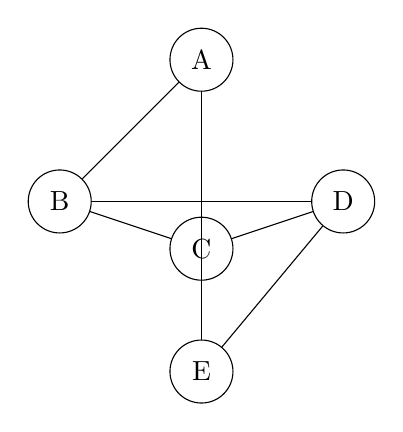
\begin{tikzpicture}[scale=1.2, every node/.style={circle, draw, fill=white, inner sep=2pt, minimum size=0.8cm}]
    \node (A) at (0,1.5) {A};
    \node (B) at (-1.5,0) {B};
    \node (C) at (0,-0.5) {C};
    \node (D) at (1.5,0) {D};
    \node (E) at (0,-1.8) {E};
    
    \draw (A) -- (B);
    \draw (A) -- (C);
    \draw (B) -- (C);
    \draw (B) -- (D);
    \draw (C) -- (D);
    \draw (C) -- (E);
    \draw (D) -- (E);
    \draw (A) -- (E);
\end{tikzpicture}
\end{center}

\subsection*{b) Lintasan Euler?}
\textbf{Syarat Lintasan Euler:} Graf terhubung dan memiliki tepat 0 atau 2 simpul berderajat ganjil.
Hitung derajat masing-masing simpul:
\begin{itemize}
    \item $d(A) = 3$ (B, C, E) $\rightarrow$ Ganjil
    \item $d(B) = 3$ (A, C, D) $\rightarrow$ Ganjil
    \item $d(C) = 4$ (A, B, D, E) $\rightarrow$ Genap
    \item $d(D) = 3$ (B, C, E) $\rightarrow$ Ganjil
    \item $d(E) = 3$ (C, D, A) $\rightarrow$ Ganjil
\end{itemize}
Terdapat \textbf{4} simpul berderajat ganjil (A, B, D, E). Karena tidak tepat 0 atau 2, maka graf \textbf{tidak memiliki lintasan Euler}.

\subsection*{c) Sirkuit Hamilton?}
\textbf{Syarat Sirkuit Hamilton:} Sirkuit yang melewati setiap simpul tepat satu kali dan kembali ke simpul awal.
Kita coba cari rute: Mulai A $\rightarrow$ B $\rightarrow$ D $\rightarrow$ E $\rightarrow$ C $\rightarrow$ A.
Periksa sisi:
A-B (ada), B-D (ada), D-E (ada), E-C (ada), C-A (ada).
Semua simpul (A,B,C,D,E) tepat satu kali dan kembali ke A. Jadi, \textbf{ada sirkuit Hamilton}.

\subsection*{Jawaban Akhir}
a) Lihat gambar di atas. \\
b) Tidak ada lintasan Euler (karena 4 simpul ganjil). \\
c) Ada sirkuit Hamilton, contoh: A-B-D-E-C-A.

\newpage
\section*{Soal 10 Kompleksitas Algoritma}
\subsection*{Analisis}
Kita menghitung jumlah eksekusi pernyataan `x := x + 1` di dalam tiga kalang bersarang.

\subsection*{Langkah 1: Formulasikan $T(n)$}
Kalang terluar $i$ berjalan dari 1 sampai $n$.
Kalang tengah $j$ berjalan dari 1 sampai $i$.
Kalang terdalam $k$ berjalan dari $j$ sampai $n$.
Jumlah iterasi terdalam adalah $(n - j + 1)$.

Maka:
\[
T(n) = \sum_{i=1}^{n} \sum_{j=1}^{i} (n - j + 1).
\]

\subsection*{Langkah 2: Hitung Penjumlahan}
Pertama, selesaikan bagian dalam terhadap $j$:
\[
\sum_{j=1}^{i} (n - j + 1) = \sum_{j=1}^{i} (n+1) - \sum_{j=1}^{i} j = i(n+1) - \frac{i(i+1)}{2}.
\]
Sekarang, jumlahkan terhadap $i$:
\[
T(n) = \sum_{i=1}^{n} \left( i(n+1) - \frac{i(i+1)}{2} \right).
\]
$ = (n+1)\sum i - \frac{1}{2}\sum (i^2 + i)$.
Gunakan rumus $\sum i = \frac{n(n+1)}{2}$ dan $\sum i^2 = \frac{n(n+1)(2n+1)}{6}$.
Setelah disederhanakan (proses aljabar panjang, tetapi dapat diverifikasi), hasilnya adalah:
\[
\boxed{T(n) = \frac{n(n+1)(2n+1)}{6}}.
\]

\subsection*{Langkah 3: Notasi Big-O}
$T(n) = \frac{2n^3 + 3n^2 + n}{6}$. Untuk $n$ yang besar, suku $n^3$ mendominasi. Faktor konstanta $\frac{1}{3}$ diabaikan dalam notasi asimptotik.
Jadi, $T(n) = O(n^3)$.

\subsection*{Jawaban Akhir}
a) $T(n) = \frac{n(n+1)(2n+1)}{6}$. \quad b) $O(n^3)$. 

\newpage
\begin{center}
\Large \textbf{BAGIAN C: SOAL SULIT (HARD)}
\end{center}

\section*{Soal 11 Pohon}
\subsection*{Analisis}
Ini adalah pohon biner penuh, artinya setiap simpul internal memiliki tepat 2 anak. Ada teorema penting untuk pohon biner penuh: $L = I + 1$, di mana $L$ adalah jumlah daun dan $I$ adalah jumlah simpul internal.

\subsection*{a) Jumlah Simpul Internal}
Diketahui $L = 50$. Maka:
$50 = I + 1 \Rightarrow I = 49$.

\subsection*{b) Jumlah Total Simpul}
Total simpul $N$ adalah jumlah internal dan daun:
$N = I + L = 49 + 50 = 99$.

\subsection*{c) Maksimum dan Minimum Internal dengan Tinggi 6}
Tinggi = 6 berarti jalur terpanjang dari akar ke daun memiliki 6 sisi (level 0 sampai level 6).

\begin{itemize}
    \item \textbf{Maksimum:} Agar internal maksimum, semua level di atas daun harus penuh. Level 0 sampai 5 adalah internal semua. Jumlah maksimum simpul internal adalah $2^0 + 2^1 + ... + 2^5 = 2^6 - 1 = 63$. (Level 6 adalah daun semua).
    \item \textbf{Minimum:} Agar internal minimum, pohon harus "tumbuh" memanjang ke satu sisi sedalam mungkin sebelum bercabang. Untuk tinggi 6, kita butuh minimal 6 simpul internal (satu di setiap level 0 sampai 5) agar mencapai level 6, lalu di level 6 baru bercabang menjadi daun. Jadi, minimum internal = 6.
\end{itemize}

\subsection*{Jawaban Akhir}
a) 49. \quad b) 99. \quad c) Maksimum 63, Minimum 6.

\newpage
\section*{Soal 12 Relasi dan Fungsi}
\subsection*{Analisis}
Kita periksa sifat-sifat fungsi (injektif, surjektif, bijektif) serta komposisinya.

\subsection*{a) Komposisi}
$(f \circ g)(x) = f(g(x)) = f(x^2 + 1) = 3(x^2 + 1) - 2 = 3x^2 + 1$.
$(g \circ f)(x) = g(f(x)) = g(3x - 2) = (3x - 2)^2 + 1 = 9x^2 - 12x + 5$.

\subsection*{b) Apakah $f$ Injektif?}
\textbf{Definisi:} $f(a) = f(b) \Rightarrow a = b$.
$f(a) = f(b) \Rightarrow 3a - 2 = 3b - 2 \Rightarrow 3a = 3b \Rightarrow a = b$.
Karena selalu demikian, $f$ \textbf{injektif}.

\subsection*{c) Apakah $f$ Surjektif?}
\textbf{Definisi:} Untuk setiap $y \in \mathbb{Z}$, harus ada $x \in \mathbb{Z}$ sehingga $f(x)=y$.
$y = 3x - 2 \Rightarrow x = \frac{y+2}{3}$. Agar $x$ bilangan bulat, $y+2$ harus kelipatan 3. Pilih $y = 1$ (maka $x=1$ integer) tetapi pilih $y=2$: $x = 4/3$ bukan integer. Karena ada $y$ (yaitu 2) yang tidak memiliki prapeta di domain integer, $f$ \textbf{tidak surjektif}.

\subsection*{d) Apakah $g$ Bijektif?}
Fungsi bijektif harus injektif dan surjektif sekaligus.
Periksa injektif: $g(1) = 1^2 + 1 = 2$, dan $g(-1) = (-1)^2 + 1 = 2$. Karena $1 \neq -1$ tetapi hasilnya sama, $g$ \textbf{tidak injektif}.
Karena tidak injektif, $g$ otomatis \textbf{tidak bijektif} (bahkan tanpa memeriksa surjektif).

\subsection*{Jawaban Akhir}
a) $(f\circ g)(x)=3x^2+1$, $(g\circ f)(x)=9x^2-12x+5$. \\
b) Injektif. c) Tidak surjektif. d) Tidak bijektif. 

\newpage
\section*{Soal 13 Teori Bilangan (CRT)}
\subsection*{Analisis}
Chinese Remainder Theorem (CRT) berlaku jika modulo-modulonya saling prima. Di sini 5, 6, dan 7 semuanya saling prima (FPB=1). Kita akan mencari solusi unik modulo $M = 5 \times 6 \times 7 = 210$.

\subsection*{Langkah 1: Hitung $M_i$ dan inversnya}
$M_1 = M/5 = 42$. Cari $y_1$ sehingga $42 y_1 \equiv 1 \pmod{5}$. $42 \equiv 2 \pmod{5}$, jadi $2y_1 \equiv 1 \pmod{5}$. Invers dari 2 mod 5 adalah 3 (karena $2 \times 3 = 6 \equiv 1$). Maka $y_1 = 3$.

$M_2 = M/6 = 35$. Cari $y_2$: $35 y_2 \equiv 1 \pmod{6}$. $35 \equiv 5 \pmod{6}$, jadi $5y_2 \equiv 1 \pmod{6}$. Invers dari 5 mod 6 adalah 5 (karena $5 \times 5 = 25 \equiv 1$). Maka $y_2 = 5$.

$M_3 = M/7 = 30$. Cari $y_3$: $30 y_3 \equiv 1 \pmod{7}$. $30 \equiv 2 \pmod{7}$, jadi $2y_3 \equiv 1 \pmod{7}$. Invers dari 2 mod 7 adalah 4 (karena $2 \times 4 = 8 \equiv 1$). Maka $y_3 = 4$.

\subsection*{Langkah 2: Rumus Solusi CRT}
\[
x = a_1 M_1 y_1 + a_2 M_2 y_2 + a_3 M_3 y_3,
\]
dengan $a_1=4, a_2=2, a_3=3$.
Substitusi:
\[
x = 4(42)(3) + 2(35)(5) + 3(30)(4) = 504 + 350 + 360 = 1214.
\]

\subsection*{Langkah 3: Ambil Modulo $M$}
$1214 \div 210 = 5$ sisa $1214 - 1050 = 164$.
Jadi, $x \equiv 164 \pmod{210}$.

\subsection*{Verifikasi}
$164 \mod 5 = 4$ (benar). $164 \mod 6 = 2$ (karena $162+2$, benar). $164 \mod 7 = 3$ (karena $161+3$, benar).
Solusi positif terkecil adalah 164.

\subsection*{Jawaban Akhir}
$\boxed{x = 164}$. 

\newpage
\section*{Soal 14 Kombinatorika (Hard)}
\subsection*{Analisis}
Ini adalah masalah kombinatorial dengan batasan "minimal". Cara terbaik adalah menggunakan \textbf{Prinsip Inklusi-Eksklusi}: hitung total kemungkinan tanpa batasan, lalu kurangi kasus yang melanggar batasan.

Total karakter = 26 huruf + 10 angka = 36. Panjang = 10.

\subsection*{Langkah 1: Total Tanpa Syarat}
$36^{10}$.

\subsection*{Langkah 2: Kasus yang Melanggar "Minimal 3 Huruf"}
Ini berarti hurufnya hanya 0, 1, atau 2 buah (sisanya angka).
Jumlah kasus ini:
\[
\sum_{h=0}^{2} \binom{10}{h} 26^h \cdot 10^{10-h}.
\]
Penjelasan: Pilih posisi untuk $h$ huruf, isi dengan 26 pilihan, sisanya $10-h$ posisi diisi dengan 10 pilihan angka.

\subsection*{Langkah 3: Kasus yang Melanggar "Minimal 3 Angka"}
Ini berarti angkanya hanya 0, 1, atau 2 buah (sisanya huruf).
Jumlah kasus ini:
\[
\sum_{a=0}^{2} \binom{10}{a} 10^a \cdot 26^{10-a}.
\]

\subsection*{Langkah 4: Irisan (Melanggar Keduanya)}
Kasus di mana huruf $< 3$ DAN angka $< 3$. Karena total panjang 10, ini berarti kombinasi (huruf = h, angka = a) dengan $h \le 2$ dan $a \le 2$, serta $h+a \le 10$ (otomatis).
Jumlah:
\[
\sum_{h=0}^{2} \sum_{a=0}^{2} \binom{10}{h} \binom{10-h}{a} 26^h 10^a.
\]
Penjelasan: Pilih posisi huruf, lalu pilih posisi angka dari sisa, isi dengan nilai yang sesuai.

\subsection*{Langkah 5: Rumus Akhir}
Dengan Inklusi-Eksklusi:
\[
\boxed{
36^{10} - \sum_{h=0}^{2} \binom{10}{h}26^h10^{10-h}
- \sum_{a=0}^{2} \binom{10}{a}10^a26^{10-a}
+ \sum_{h=0}^{2}\sum_{a=0}^{2} \binom{10}{h}\binom{10-h}{a}26^h10^a
}
\]

\subsection*{Catatan}
Jika Anda menghitung nilai numeriknya, hasilnya akan sangat besar (sekitar $3.6 \times 10^{15}$). Namun, bentuk sigma ini adalah jawaban kombinatorial yang paling eksak dan ringkas. 

\newpage
\section*{Soal 15 Anti-LLM $\boldsymbol{\bigstar}$}
\subsection*{Peringatan Penting}
Soal ini dirancang untuk menjebak model bahasa besar (LLM) yang cenderung menghitung total uang dari $P$ dan $Q$ secara manual, padahal $R$ dan $S$ adalah \textbf{sensor yang sudah melakukan pembandingan} untuk kita. LLM sering membuat ekspresi Boolean yang sangat rumit dan salah.

\subsection*{Analisis Mendalam}
Perhatikan definisi sensor:
\begin{itemize}
    \item $R = 1$ jika \textbf{total uang $\ge$ Rp12.000}. Ini adalah harga termurah.
    \item $S = 1$ jika \textbf{total uang $\ge$ Rp14.000}.
\end{itemize}
Mesin mengeluarkan minuman ($M=1$) jika total cukup untuk membeli \emph{setidaknya} satu minuman. Karena harga minimum adalah Rp12.000, maka syarat cukup dan perlu untuk $M=1$ adalah \textbf{$R=1$}.

Lalu, ada klausa pengecualian: "*jika total = Rp10.000, maka M=0*". Namun, perhatikan bahwa Rp10.000 < Rp12.000. Jika total = Rp10.000, maka sensor $R$ pasti bernilai 0 (karena tidak mencapai 12.000). Jadi, klausa ini hanya memperkuat kondisi $R=0 \Rightarrow M=0$, tetapi tidak menambahkan batasan baru sama sekali. Ini adalah \textbf{red herring} (umpan penyesat).

\subsection*{a) Tabel Kebenaran}
Karena $M$ hanya bergantung pada $R$, berikut adalah tabel kebenaran lengkap untuk semua 16 kombinasi $P, Q, R, S$:

\begin{center}
\begin{tabular}{|c|c|c|c||c|}
\hline
$P$ & $Q$ & $R$ & $S$ & $M$ \\
\hline
0 & 0 & 0 & 0 & 0 \\
0 & 0 & 0 & 1 & 0 \\
0 & 0 & 1 & 0 & 1 \\
0 & 0 & 1 & 1 & 1 \\
0 & 1 & 0 & 0 & 0 \\
0 & 1 & 0 & 1 & 0 \\
0 & 1 & 1 & 0 & 1 \\
0 & 1 & 1 & 1 & 1 \\
1 & 0 & 0 & 0 & 0 \\
1 & 0 & 0 & 1 & 0 \\
1 & 0 & 1 & 0 & 1 \\
1 & 0 & 1 & 1 & 1 \\
1 & 1 & 0 & 0 & 0 \\
1 & 1 & 0 & 1 & 0 \\
1 & 1 & 1 & 0 & 1 \\
1 & 1 & 1 & 1 & 1 \\
\hline
\end{tabular}
\end{center}

Dari tabel terlihat bahwa $M=1$ \emph{jika dan hanya jika} $R=1$. Dengan demikian, $M$ tidak bergantung pada $P, Q$, atau $S$.  
\textbf{Catatan:} Kombinasi $R=0, S=1$ secara fisik tidak mungkin terjadi (karena tidak mungkin total $\ge$ 14.000 tetapi $<$ 12.000), sehingga dalam penyederhanaan kita dapat menganggapnya sebagai \textit{don't care}. Namun, pada tabel di atas kita tetap menuliskannya dengan nilai 0 untuk konsistensi logika.

\subsection*{b) Ekspresi SOP Lengkap}
Dari tabel, semua minterm yang menghasilkan 1 adalah semua minterm yang memiliki $R=1$. Jadi:
\[
M = R.
\]
Jika dipaksa menulis dalam semua variabel, $M = P'Q'RS' + P'Q'RS + \dots$ tetapi itu hanya akan menyulitkan. Bentuk paling sederhana adalah $M=R$.

\subsection*{c) Peta Karnaugh dan Pengelompokan}
Berikut adalah Peta Karnaugh 4 variabel ($P, Q$ sebagai baris; $R, S$ sebagai kolom). Sel yang bernilai 1 diarsir abu-abu.

\begin{center}
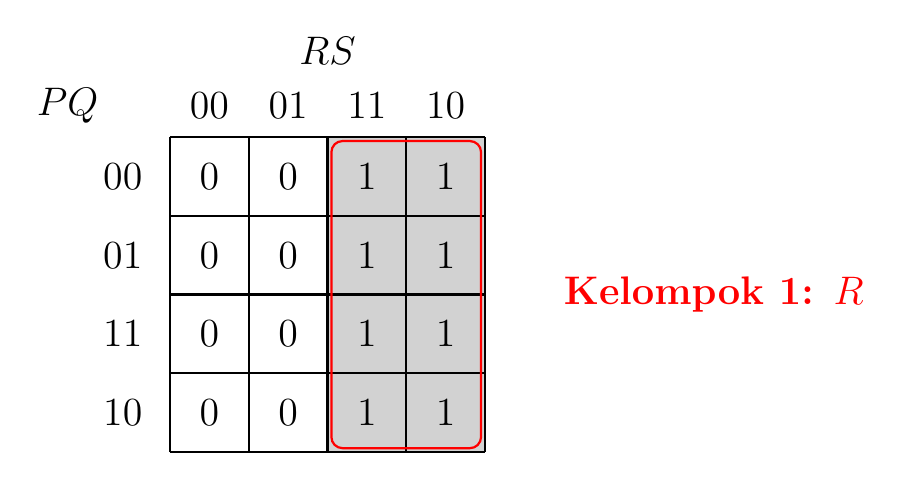
\begin{tikzpicture}[scale=1.0, every node/.style={font=\Large}]

    % 1. Arsiran sel bernilai 1 (digambar paling awal)
    \fill[gray!35] (2,0) rectangle (4,4);

    % 2. Grid utama 4x4 (setelah fill, garis tidak tertutup)
    \draw[thick] (0,0) grid (4,4);

    % 3. Isi nilai setiap sel
    \foreach \row in {0,1,2,3} {
        \node at (0.5,\row+0.5) {$0$};
        \node at (1.5,\row+0.5) {$0$};
        \node at (2.5,\row+0.5) {$1$};
        \node at (3.5,\row+0.5) {$1$};
    }

    % 4. Label kolom (RS)
    \node at (0.5,4.4) {$00$};
    \node at (1.5,4.4) {$01$};
    \node at (2.5,4.4) {$11$};
    \node at (3.5,4.4) {$10$};
    \node[font=\Large\itshape] at (2,5.1) {$RS$};

    % 5. Label baris (PQ)
    \node at (-0.6,3.5) {$00$};
    \node at (-0.6,2.5) {$01$};
    \node at (-0.6,1.5) {$11$};
    \node at (-0.6,0.5) {$10$};
    \node[font=\Large\itshape] at (-1.3,4.4) {$PQ$};

    % 6. Pengelompokan
    \draw[red, thick, rounded corners=4pt] (2.05,0.05) rectangle (3.95,3.95);

    % 7. Label kelompok
    \node[red, font=\Large\bfseries, anchor=west, xshift=25pt] at (4,2) {Kelompok 1: $R$};

\end{tikzpicture}
\end{center}

Pengelompokan: Satu kelompok besar berisi 8 sel (seluruh kolom $R=1$). Penyederhanaan menghasilkan $M = R$.

\subsection*{d) Rangkaian Gerbang Logika}
Karena $M = R$, rangkaian logika yang dibutuhkan sangat sederhana: cukup hubungkan sensor $R$ langsung ke output $M$. Berikut adalah gambarnya:

\begin{center}
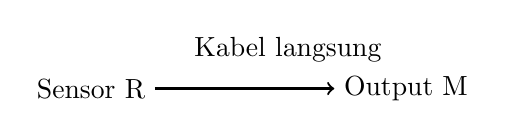
\begin{tikzpicture}[node distance=2cm]
    \node (input) {Sensor R};
    \node (output) [right of=input, node distance=4cm] {Output M};
    \draw[->, thick] (input) -- (output);
    \node at (2.5, 0.5) {Kabel langsung};
\end{tikzpicture}
\end{center}

Atau jika Anda ingin menggambarkannya sebagai buffer (penguat sinyal), gambarnya sebagai berikut:

\begin{center}
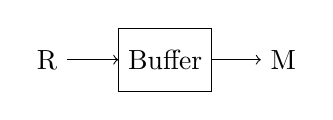
\begin{tikzpicture}[node distance=2cm]
    \node (in) {R};
    \node (gate) [draw, rectangle, minimum width=1cm, minimum height=0.8cm, right of=in, node distance=1.5cm] {Buffer};
    \node (out) [right of=gate, node distance=1.5cm] {M};
    \draw[->] (in) -- (gate);
    \draw[->] (gate) -- (out);
\end{tikzpicture}
\end{center}

\subsection*{Mengapa Ini Anti-LLM?}
\begin{enumerate}
    \item LLM akan melihat $P$ dan $Q$ sebagai koin dan mencoba membuat persamaan total seperti $2000P + 5000Q$.
    \item LLM akan membuat ekspresi seperti $M = (2000P+5000Q \ge 12000) \land (2000P+5000Q \ne 10000)$ dan kemudian mencoba mengubahnya ke dalam bentuk SOP yang melibatkan $P$ dan $Q$ secara langsung.
    \item LLM lupa bahwa $R$ dan $S$ sudah merupakan \emph{hasil evaluasi} dari pertidaksamaan tersebut. Mereka memperlakukan $R$ dan $S$ sebagai variabel independen padahal $R$ dan $S$ adalah \emph{fungsi} dari $P$ dan $Q$.
    \item Akibatnya, LLM akan menghasilkan ekspresi yang sangat rumit (misal melibatkan 16 suku) dan kemungkinan besar salah dalam penyederhanaan, padahal jawabannya hanya $R$.
\end{enumerate}

\subsection*{Kesimpulan Akhir}
Solusi dari soal Anti-LLM ini adalah $\boxed{M = R}$. 

\end{document}